\documentclass[12pt,a4paper]{article}

\usepackage[margin=1in]{geometry}
\usepackage[english]{babel}
\usepackage[T1]{fontenc}
\usepackage[utf8]{inputenc}

\usepackage{longtable}
\usepackage{tabularx}
\usepackage{booktabs}
\usepackage{array}
\usepackage{multirow}
\usepackage{graphicx}
\usepackage{xcolor}
\usepackage{enumitem}
\usepackage[parfill]{parskip}
\usepackage[title,titletoc]{appendix}
\usepackage{amsmath}
\usepackage{fnpos}
\usepackage{geometry}
\usepackage{csquotes}
\usepackage{tikz}
\usepackage{pdflscape}

\usetikzlibrary{positioning}
\usetikzlibrary{calc}
 \tikzstyle{main} = [rectangle, rounded corners, minimum height=0.7cm,text centered, draw=black, font=\scriptsize]
 \tikzstyle{process} = [rectangle, minimum height=0.7cm, text centered, draw=black, font=\scriptsize]
 \tikzstyle{note} = [rectangle, text centered, minimum height=1cm]
 \tikzstyle{arrow} = [->,>=stealth,auto,font=\scriptsize,node distance=3cm, main node/.style={circle,draw}]

\usepackage[hyphens]{url}

\usepackage[backend=biber,url=false,style=authoryear,sorting=nyt,bibstyle=numeric]{biblatex}
\addbibresource{chequeBounce.bib}

\usepackage[acronym,nonumberlist,nomain]{glossaries}
\makeglossary
\loadglsentries{acronyms.tex}

\AtBeginEnvironment{quote}{\smaller}
\makeFNbottom
\geometry{margin=1in}
\renewcommand{\baselinestretch}{1.25}
\setlength{\parskip}{1em}
\setlist{nosep}

\newcommand{\floattabu}[1]{
\vspace*{0.2in}
{\footnotesize
#1
}
\vspace*{0.2in}}


\usepackage[hidelinks,breaklinks]{hyperref}
\usepackage{cleveref}

\title{Characterising cheque dishonour cases in India: Causes for delays and policy implications}
\author{Devendra Damle\thanks{Devendra Damle is a researcher at National Institute of Public Finance and Policy.} and Jitender Madaan\thanks{Jitender Madaan is a professor at Indian Institute of Technology, Delhi.} and Karan Gulati\thanks{Karan Gulati is a researcher at the Vidhi Centre for Legal Policy.}\\ and Manish Kumar Singh\thanks{Manish Kumar Singh is a professor at Indian Institute of Technology, Rourkee.} and Nikhil Borwankar\thanks{Nikhil Borwankar is a practicing advocate.}}

\begin{document}
\maketitle

\begin{abstract}
TO DO
\end{abstract}

\newpage
\tableofcontents
\newpage
\printglossaries
\listoftables
\newpage

\section*{Acknowledgements}
The authors would like to thank the DAKSH Centre of Excellence for Law and Technology for their support. The authors are grateful to thank Sandhya PR and Surya Prakash BS (both from DAKSH) for their extensive feedback on the study. The authors would also like to thank Manaswini Rao (Professor of Economics, University of California San Diego) and Pramod Rao (Group General Counsel, ICICI Group) for reviewing the study and their inputs.

\newpage
\section{Introduction}
\label{sec:introduction}
India has a slow judiciary - courts are clogged with large backlogs \autocite{moog1992delays, debroy2008justice, dutta2019modernise}. As of 8th December 2021, over forty-one million cases were pending across district courts \autocite{njdg2021}. Slow judiciaries have adverse consequences on the structure and efficiency of markets and the quality of life of citizens \autocite{world2004world, chemin2007impact, rao2020institutional}. Therefore, minimising unnecessary judicial delays could help improve enforcement and enhance the overall rule of law. It is estimated that judicial delays cost India around 1.5\% of its GDP annually.\footcite{dey2016_cost} Against this backdrop, it is hardly surprising that tackling judicial delay has increasingly become a top priority for Indian judges and policymakers.

One reason for the large burden on courts is believed to be the (supposed) large share of \gls{ni} cases.\footnote{In particular, \S~138 of the Negotiable Instruments Act (Dishonour of cheque for insufficiency, etc., of funds in the account). Act 26 of 1881} As per the \gls{lci}, they represent 6.5\% and 7.8\% of all institutions and pendency in Indian courts, respectively \autocite{lci2014_arrears}. As per one order of the Supreme Court of India, they reflect more than 15\% of all criminal cases in the District Courts \autocite{sc2020_makwanavstate}. As per another order, they constitute 30\% of the total pendency in courts.\footcite[Similarly, a study published by the Department of Justice briefly touches on the burden of such cases on the judiciary and posits that they constitute 34\% of pending criminal cases in Maharashtra.][]{sc2020_138, mahadik2018_maharashtra}

Given the disagreement, any acceptance among policymakers that \gls{ni} cases (\textit{cheque dishonour cases} hereinafter) are the reason for India's slow judiciary is likely to lead to misguided solutions. The misrepresentation could lead to diverting resources from other routes of judicial reform. Thus, one requires a more detailed analysis of the proportion of such cases, their causes, timelines, etc. This information can help judges and policymakers better target interventions.\footcite[For the importance of accurate judicial data, see][]{damle2020_ecourtsData, daksh2020_data, damle2020_land}

To this end, in 2020, the Supreme Court of India took on board a suo-motu case concerning the “expeditious trial of cases under section 138 of the Negotiable Instruments Act 1881” \autocite{sc2020_138}. Among other directions, the court (i) appointed a \gls{coe}\footnote{Headed by Hon’ble Mr Justice RC Chavan, former Judge of the Bombay High Court.} and (ii) appointed Amici Curiae to assist the court,\footnote{Mr Sidharth Luthra (Sr Advocate) and Mr K Parameshwar (Advocate).} to study processes to expedite disposal of complaints under \S~138 of the \gls{ni}. This is in a series of interventions targeted to understand cheque dishonour cases in India. As \cref{sec:history} shows, most knowledge and development concerning such cases in India has come from government institutions, i.e. the \gls{lci} and the judiciary.

Such knowledge is based on the assumption that cheque dishonour cases are a large burden on the judiciary and has thus focused on expediting disposal. For example, \gls{lci} (2008), by relying on newspaper reports concerning the proportion of cheque dishonour cases, recommended setting up Fast Track Magisterial Courts \autocite{lci2008_138, bhan2015_placing}. However, it did not define \textit{fast-track courts} or give guidance concerning how and where they would operate. Developing this work, DAKSH (2017) examined the behaviour of cheque dishonour cases in the Indian courts by looking at over 67000 cases. In most cases, it found that resolution is delayed well beyond statutorily prescribed timelines and that certain banks and financial institutions are frequent complainants \autocite{sridhar2017_cheque}.

In 2020, the Amici appointed by the Supreme Court also made recommendations to expedite the disposal of cases. This included (i) increasing the use of pre- and post-summons mediation, (ii) expediting the service of summons to reduce absconsion, (iii) addressing the multiplicity of proceedings, etc.\footcite[For details see ]{amicus2020_submission} This study, based on orders of the Supreme Court and the report of the Amici Curiae, attempts to assess the effect of suggested interventions on the expeditious trial of cases under \S~138 of the \gls{ni}. It first answers important questions regarding the volume of such cases across differing courts. It then examines the determinants of case duration as identified by the Amici Curiae and the Supreme Court.

The rest of this paper is organised as follows: after this introduction, \cref{sec:history} elaborates the history of cheque dishonour provisions in India and their relation with judicial delays. \Cref{sec:methodology} describes the methodology, and \cref{sec:results} presents the results thereof. Finally, \cref{sec:conclusion} concludes the paper and presents the way forward.

\section{Cheque dishonour and judicial delays} \label{sec:history}

The \acrlong{ni} was enacted to define the law relating to promissory notes, bills of exchange, and cheques (for an explanation of \S~138, see Appendix \ref{app:understanding}).\footcite[See for details][]{ind1881_niAct} To increase the culture regarding the use of cheques, the Act was amended in 1988.\footcite{niAmend1988} A new chapter (\S\S~138 to 142) was incorporated for penalties in the event of dishonour of cheques due to insufficient funds in the account of the drawer of the cheque. \S~138 provided for the circumstances under a drawer can be penalised for the dishonour of a cheque.

However, by 2001, these provisions were thought not to have had the desired effect \autocite{stdcomm2001_138niAct}. While the punishment was thought to be inadequate, courts could not dispose of cases in a time-bound manner due to the large number of cases pending across the country. Given the large burden on courts, a Working Group was constituted the same year to review \S~138 of the \gls{ni} and make recommendations regarding the changes needed to effectively achieve the purpose of the section \autocite{wg2001_138}. In light of the recommendations of the Working Group, the government decided to bring further amendments to the Act. Among others, the amendments included:

\begin{enumerate}[label=(\alph*)]
 \item increasing the punishment from one year to two years;
 \item providing discretion to the court to waive the period of one month for taking cognisance of a case;
 \item prescribing the procedure for dispensing with preliminary evidence of the complainant;
 \item prescribing the procedure for service of summons via speed post or impanelled private couriers;
 \item providing for summary trials; and
 \item making the offence compoundable.
\end{enumerate}

The amendments were considered by the Lok Sabha Standing Committee on Finance, which recommended that given the large burden on courts, the proposed amendments be coupled with the creation of specialised courts for \S~138 cases \autocite{stdcomm2001_138niAct}. However, the subsequent Amending Act did not reference specialised courts.\footcite[See ][]{niAmend2002} The Act was also amended in 2015 and 2018 to clarify the appropriate area of jurisdiction where cheque dishonour cases can be filed, and grant power to courts to grant interim compensation, respectively.\footcite[For details see][]{niAmend2015, niAmend2018}

\gls{lci} took up the proposal for specialised courts in 2008. According to the Commission, the credibility of the financial sector was facing setbacks due to the large pendency of dishonoured cheque cases. Relying on an array of judgments by the Supreme Court of India concerning speedy trials the Commission recommended the introduction of fast track courts to address cases concerning dishonour of cheques under \S~138 of the Act.\footcite[See for details ][]{sc1978_khatoon, sc1981_champalal, sc2005_surinder, sc2008_krishna} However, it did not comment on the number or expected workload of such courts \autocite{lci2008_138}. The need for additional courts was re-iterated by \gls{lci} in 2009 \autocite{lci2009_reforms}.

While \gls{lci} has focused on the need for more courts, the Supreme Court has provided assistance in implementing the amendments. In 2014, noting that the prime reason for the delays in \S~138 case is the absence of the accused, the Court held that the magistrate should adopt a pragmatic and realistic approach such as issuing notices and summons via e-mail or push notification to ensure delivery.\footcite[See ][]{sc2014_iba} In 2018, the court directed banks to give the details of the e-mail of the accused to the complainant for service through e-mail. The court also directed that: (i) cases must be dealt with summarily, (ii) the evidence of the complainant must be conducted within three months, (iii) an endeavour must be made to conclude the trial within six months, (iv) the trial, as far as practicable, must be held on a day-to-day basis, and (v) High Courts may pass additional localised directions for speedy disposal of cases.\footcite[See ]{sc2018_meters}

Lastly, in March 2020, the Supreme Court of India took on board a suo-motu case concerning the “expeditious trial of cases under section 138 of the Negotiable Instruments Act 1881”.\footcite[See ]{sc2020_138} As mentioned, the court-appointed Amici Curiae to assist in the matter, which presented its preliminary report to the court in October of the same year. The Amici made several suggestions to expedite trial, which among others, includes:

\begin{enumerate}[label=(\alph*)]
 \item Address jurisdictional issues;
 \item Address multiplicity of proceedings; and
 \item Expedite service of summons to reduce absconsion;
 \item Explore setting up specialised courts;
 \item Increase the use of pre- and post-summons mediation;
 \item Mandate presenting of a plausible defence before conversion from summary to summons trial; and
 \item Summon witnesses only when the accused presents a defence.\footcite{amicus2020_submission}
\end{enumerate}

Noticeably, the recommendations of the Amici Curiae were in line with previously accepted reasons for delays in disposal. While considering the recommendations, the Supreme Court recommended the Government and High Courts take necessary action where possible and held that they should be the subject matter of deliberation by the \gls{coe} appointed in the same case.\footnote{Headed by Hon’ble Mr Justice RC Chavan, former Judge of the Bombay High Court.}

\section{Conceptual framework and hypotheses}
\label{sec:select-case-char}

The recommendations of the Amici Curiae and the Supreme Court target several aspects of a \gls{ni} case. They posit that these aspects likely lead to delays. This study examines six areas that are the targets of these interventions, viz. ---

\begin{enumerate}
\item non-appearance by the accused;
\item trials being run as summons trials;
\item reference to mediation;
\item jurisdictional issues;
\item multiplicity of proceedings;
\item setting up additional \gls{ni} courts.
\end{enumerate}

The case characteristics whose impact we have chosen to examine were determined based on two factors: (1) the importance of that characteristic and (2) the feasibility of finding reliable information about it in the eCourts data. Accordingly, we chose to examine the effect of six case characteristics that map onto the six intervention targets mentioned above. The characteristics we chose are as follows:
\begin{enumerate}
\item The accused fails to appear before the court for at least one hearing;
\item The case is converted to a summons trial;
\item The case is referred to mediation;
\item The case has jurisdictional issues and is transferred to another court, as a result;
\item The case contains a multiplicity of proceedings --- either the dishonoured cheque was issued to satisfy multiple transactions, or multiple cheques were dishonoured;
\item The case was contested.
\end{enumerate}

These characteristics represent six kinds of events that can take place in the course of litigating the case.\footnote{These are not mutually exclusive. One or more of these events can occur in the same case.} We test whether the event's occurrence affects the case duration and the number of hearings required to dispose it. Table \ref{tab:expected} presents a summary of the expected effects of the identified case characteristics. We discuss the salience of each case characteristic and the accompanying hypotheses below.

\begin{longtable}{@{}lcc@{}}
\caption{Expected effects of case characteristics}
\label{tab:expected}\\
\toprule
\multicolumn{1}{c}{\multirow{2}{*}{\textbf{Case characteristic}}} & \multicolumn{2}{c}{\textbf{Expected effect}} \\ \cmidrule(l){2-3} 
\multicolumn{1}{c}{} & \textbf{Duration} & \textbf{Hearings} \\ \midrule
Non-appearance of the accused & + & + \\
Conversion to summons trial & + & + \\
Mediation & - & - \\
Jurisdictional issues & + & + \\
Multiplicity of proceedings & + & + \\
Contested cases & + & + \\ \bottomrule
\end{longtable}

\subsection{Non-appearance of the accused} 
\label{sec:non-appe-accus}

\textcite{ostrom2000efficiency}, in a study of nine state criminal trial courts in the United States, find that criminal cases where the defendant absconds take 40--90 days longer to dispose than those where the defendant appears in court.\footnote{The authors attribute this to the fact that in such cases, a separate procedure has to be conducted for the judge to issue a bench warrant to produce the accused before the court.} The defendant failing to appear in court is one of the leading causes for failed hearings. Consequently, delays in case disposal in the United Kingdom \autocite{crownProsecutionService2006_magistrateCourtEfficiency}. Similarly, \textcite{llangasinghe1988_fijiJudicialDelays} found that the accused absconding is the most common reason for delays in case disposal in magistrates' courts in Fiji. The Amici Curiae and the Supreme Court's recommendations are premised on the notion that non-appearance of the accused leads to delays. We, therefore, seek to examine whether this holds good for cheque dishonour cases in India. We test the following hypotheses:

\begin{description}
\item[H$_{1a}$]: cases, where the accused does not appear for one or more hearings, require more days to dispose
\item[H$_{1b}$]: cases, where the accused does not appear for one or more hearings, require more hearings to dispose
\end{description}

\subsection{Conversion to summons trial}
\label{sec:conv-summ-trial}

We could not find empirical studies on the effectiveness of summary trials in reducing case duration. Procedural law governing summary trials in the United States and United Kingdom are premised on the assumption that summary trials would reduce time delays in case disposal \autocite{miller2003}. At the same time, \textcite{miller2003} argues that regardless of the time-savings that may (or may not) result from summary trials, the discretion it gives to courts violates the principle of the right to a trial by jury. Therefore, bearing in mind the Supreme Court and Amici Curiae's recommendation that, to the extent possible, cases should be conducted as summary trials, and they should be converted to summons trials only in specific situations we test the following hypotheses:

\begin{description}
\item[H$_{2a}$]: cases converted to summons trials require more days to dispose
\item[H$_{2b}$]: cases converted to summons trials require more hearings to dispose
\end{description}

\subsection{Cases referred to mediation by the court} \label{sec:furth-exam-cases}

\textcite{buscaglia1997_latinAmericaCourtDelays} find that, in Latin American courts, when judges mandate mediation, it reduces the overall time required to dispose a case.\footnote{They conjecture is that the efficiency gains would result in judges having to dedicate less time to adjudicate such cases.} However, a review of empirical research on the time and cost-effectiveness of court-annexed Alternative Dispute Resolution (ADR), including mediation, by \textcite{wissler2004effectiveness} finds no conclusive relationship between the time required to dispose cases via ADR as compared to going to trial. Some studies reviewed by \textcite{wissler2004effectiveness} find that mediation can increase the duration. Some find that it can decrease the duration, while some find no effect. \textcite{heise2010adr} further finds that participation in ADR does not significantly affect case disposal time. However, cases where the parties choose to settle take less time than ADR. Given the mixed findings on the effect of mediation and the Supreme Court and Amici Curiae's opinion that court-annexed mediation can reduce time to dispose cases, we test the following hypotheses:

\begin{description}
\item[H$_{3a}$]: cases referred to mediation require more days to dispose
\item[H$_{3b}$]: cases referred to mediation require more hearings to dispose
\end{description}

\subsection{Jurisdictional issues}

Prima facie, there are four territorial areas involved in a cheque dishonour case - (i) where the issuer ordinarily resides, (ii) where the payee ordinarily resides, (iii) where the cheque was issued, and (iv) where the cheque was presented. 

Prior to 2015, the \gls{ni} only specified circumstances under which complaints concerning cheque dishonour could be filed. It did not specify the territorial jurisdiction of the courts where such a complaint had to be filed. This resulted in individuals filing cases in locations not readily accessible to the opposite party. Thus, cases would have to be transferred to suitable courts for hearing. In 2015, the Act was amended to provide that complaints can only be filed in a court in whose jurisdiction the bank branch of the payee lies.\footcite{niAmend2015} While this addressed the lack of clarity in the court where complaints had to be filed, invariably, cases commenced in territorial jurisdiction where the accused did not ordinarily reside.\footcite{amicus2020_submission}

Such jurisdictional issues, where cases have to be transferred from one court to another, may lead to delays.\footcite{sc2020_138, amicus2020_submission} We thus test the following hypotheses:

\begin{description}
\item[H$_{4a}$]: Cases with jurisdictional issues require more days to dispose
\item[H$_{4b}$]: Cases with jurisdictional issues require more hearings to dispose
\end{description}

\subsection{Multiplicity of proceedings}

\S~219 of the \gls{crpc} provides that when a person is accused of more than one offence of the same kind committed within twelve months, all offences may be tried together, subject to a maximum of three such offences. Similarly, as per \S~220, if a person commits more than one offence in one transaction, she may be charged with all offences and tried at one trial. Experience has shown that a single financial transaction may lead to the dishonour of multiple cheques. However, under the \gls{crpc}, only three offences and, therefore, the dishonour of only three cheques can be tried together. This has resulted in multiple proceedings involving either the same issuer (accused) or the same transaction. Reducing such multiplicity may reduce the burden on courts. We thus test the following hypotheses:

\begin{description}
\item[H$_{5a}$]: Cases involving a multiplicity of proceedings require more days to dispose
\item[H$_{5b}$]: Cases involving a multiplicity of proceedings require more hearings to dispose
\end{description}

\subsection{Contested cases}
\label{sec:contested_cases_meth}
When cases are contested, parties lead evidence before a court and rebut arguments. This is likely to lead to longer proceedings since courts have to come to reasoned decisions based on the proceedings. On the other hand, uncontested cases use minimal court resources, since parties reach a mutually acceptable decision verified by the court. \textcite{ostrom2000efficiency} find that cases that went to trial took 53--158 days longer to dispose than cases where the defendant pleaded guilty.\footnote{The variation in the average delay is between the different jurisdictions studied.} \textcite{buscaglia1997_latinAmericaCourtDelays}, in a study of judicial efficiency in Latin American courts, find that willingness to litigate increases the duration of court cases and results in a greater backlog of cases. \textcite{crownProsecutionService2006_magistrateCourtEfficiency} finds that, in magistrate courts in the United Kingdom, contested cases typically take a greater number of hearings to dispose than uncontested cases. Contested cases take longer to dispose than uncontested cases. The difference between the time it takes the courts to dispose of uncontested cases compared to contested cases can yield insights into how efficient the court is at handling cases that go to trial, compared to cases where the defendant is willing to settle or compound. The potential effectiveness of the Supreme Court and Amici Curiae's recommendation of setting up more \gls{ni} courts can be indirectly tested through this characteristic. We thus test the following hypotheses:

\begin{description}
\item[H$_{6a}$]: Contested cases require more days to dispose
\item[H$_{6b}$]: Contested cases require more hearings to dispose
\end{description}

%%% Local Variables:
%%% mode: latex
%%% TeX-master: "paper_chequeDishonour"
%%% End:

\section{Methodology}
\label{sec:methodology}
\subsection{Data description}
\label{sec:data-description}
We first drew a random sample of 100,000 cases filed between 2014/01/01 and 2018/12/31 across India from the database published by Development Data Lab.\footcite{devdatalabs2021_eCourtsData} We then attempted to download the case-details for these 100,000 cases from the eCourts database. We were able to download case-details for approximately 89,000 cases. We used regular expressions to check whether the ``Act Name'' field references the \gls{ni}. Then, we used regular expressions to search for references to the \gls{ni} in the interim and final order texts, where available. We tagged the cases we found through this protocol as related to the \gls{ni}. Data availability and quality vary greatly across states. Consequently, we could not include all the states of India in our study. We identified the states to exclude from the study based on the following criteria:

\begin{itemize}
\item States/Union Territories where we were unable to download sample data (this is because of data quality of the e-courts database);
\item States/Union Territories that do not classify any cases as relating to the Negotiable Instruments Act;
\item States/Union Territories where < 2\% of the final orders (as a proportion of total NI cases) are machine-readable and in English.
\end{itemize}

Based on the aforementioned criteria, of the 29 states (including Jammu and Kashmir) and 7 Union Territories, we dropped 21 states and 5 Union Territories. Our final sample covers 8 states and 2 Union Territories, shown in Table \ref{tab:sample_desc}. For these 10 states and Union Territories, we drew a random sample of 500,000 cases from the Development Data Labs database.\footcite{devdatalabs2021_eCourtsData} We then attempted to download case details for these 500,000 cases filed between 2014/01/01 and 2018/12/31. We were able to successfully download case-details for 4,68,855 cases. We removed cases from District and Sessions courts since these courts hear appeals, and we are only interested in original matters. This gave us a sample of 3,63,762 cases. As with the preliminary analysis, we used pattern-matching based on regular expressions to identify cases related to \gls{ni}. In total, our sample has 48,191 \gls{ni} cases. Out of these, 10,693 are pending cases and 37,498 are disposed. Table \ref{tab:sample_desc} shows a summary of the sample. Our data shows that check-dishonour cases in India represent approximately 13.2\% of all court cases (pending+disposed).

{\footnotesize \begin{longtable}{@{}lrrrr@{}}
\caption{Sample description}
\label{tab:sample_desc}\\
\toprule
\textbf{State} & \textbf{\gls{ni} cases} & \textbf{\%\gls{ni} cases} & \textbf{Non-\gls{ni} cases} & \textbf{Total cases}\\ \midrule
\endhead
Andhra Pradesh & 2640 & 12.4 & 18567 & 21207\\
Chandigarh & 731 & 34.9 & 1364 & 2095\\
Delhi & 5211 & 26.1 & 14742 & 19953\\
Goa & 399 & 12.8 & 2713 & 3112\\
Gujarat & 6756 & 12.0 & 49476 & 56232\\
Haryana & 5326 & 13.7 & 33542 & 38868\\
Himachal Pradesh & 1166 & 8.9 & 11948 & 13114\\
Karnataka & 11195 & 12.9 & 75807 & 87002\\
Maharashtra & 8880 & 9.7 & 82673 & 91553\\
Punjab & 5887 & 19.2 & 24739 & 30626\\
\textbf{Total} & \textbf{48191} & \textbf{13.2} & \textbf{315571} & \textbf{363762}\\ \bottomrule
\end{longtable}
}

\subsection{Approach to analysis}
\label{sec:approach-analysis}

Our objective is two-fold, to examine whether the interventions proposed by the Amicus Curiae are likely to affect the duration of cheque-dishonour cases, and if so what is the magnitude of the effect. To that end, we first identified cases with specific characteristics that are thought to increase the duration of a cheque-dishonour case. We then used a fixed-effects regression model to estimate the size of the effect of each of these characteristics on the total duration of the case. For the empirical analysis, we only used the 37,498 disposed cases.

\subsubsection{Text-mining}
\label{sec:text-mining}

We used pattern-matching based on regular expressions on the texts of the interim and final orders for each case to identify cases with the characteristics of interest. We supplemented this with the information reported in the purpose of hearings and the nature of disposal. The characteristics and the strategy to identify whether it applies to a given case are as follows:

\begin{description}
\item [Non-appearance by the accused] -- We looked for references to Section 72
  CrPC, terms like accused not available / out of station / absconding
  / not present / absent, or that accused’s presence could not be
  secured, or references to the issuance of a bailable / non-bailable
  warrant to secure the presence of the accused. In addition to this,
  we looked at references to non-appearance, absconsion, bailable /
  non-bailable warrants in the data on the purpose of hearings.
\item [Jurisdiction issue] -- We looked for references to lack of
  jurisdiction / lack of proper jurisdiction / beyond jurisdiction,
  references to section 142 of the NI Act, and citations of specific
  cases like Vijay Dhanuka, KS Joseph vs Phillips
  Carbon. Additionally, we also marked cases that had been
  transferred, since a vast majority of these cases get transferred
  because of jurisdictional issues, and cases marked as transferred in
  the hearings data and disposal data.
\item [Case referred to mediation] -- We looked for references to the case being
  referred to mediation / Lok Adalat / ADR, or references to the
  matter being settled mutually, or compromised. We also looked at
  references to the cases being sent to mediation in the hearings
  data, and references to the case concluding in the Lok Adalat or
  being settled mutually, or the parties reaching a compromise.
\item [Multiplicity of proceedings] -- We looked for references to multiple cheques being dishonored and multiple transactions, and references to Section 219 and/or Section 220 of the CrPC.
\item [Case being converted to a summons trial] -- We looked for references to the case being
  tried under section 143 of the NI Act, or Sections 262, 263, 264 or
  265 of the CrPc were marked, or these sections being applicable, or
  references to the case being tried summarily were marked as not
  summons trials. Cases where these were deemed not to apply, or
  the case was being conducted normally, or it is undesirable to try
  the case summarily, or the aforementioned sections not being
  applicable were marked as summons trials. Further, cases, where any hearing mentioned summons trial as the purpose were marked as summons cases.
\end{description}

These case characteristics are represented as
binary variables. As an example, if in a given case, if the parties
did not appear for a hearing, the Non-appearance variable takes the
value 1. If the parties appeared at every hearing, we mark it as
0. Similarly, for the Summons Trial variable, if the case was
converted to a summons trial, it is marked as 1. Otherwise, it is
marked as 0. Table \ref{tab:case_chars} shows the state-wise number of
cases in which we were able to identify characteristics of interest.

{\footnotesize \centering
  \begin{longtable}{@{}lrrrrrr@{}}
  \caption{\mbox{Number of cases in which we were able to identify
    characteristics of interest}}
  \label{tab:case_chars}\\
  \toprule
  \textbf{State} & \textbf{Non} & \textbf{Summons} & \textbf{Mediation} & \textbf{Jurisdiction} & \textbf{Multiplicity} & \textbf{Total} \\
   & \textbf{Appearance} & \textbf{Trial} & & \textbf{Issue} & & \\
  \midrule
  \endhead
  Andhra Pradesh & 1674 & 814 & 260 & 210 & 124 & 2640 \\
  Chandigarh & 701 & 408 & 204 & 278 & 53 & 731 \\
  Delhi & 2062 & 1359 & 1026 & 1045 & 208 & 5211 \\
  Goa & 381 & 78 & 90 & 33 & 18 & 399 \\
  Gujarat & 5125 & 391 & 402 & 3059 & 107 & 6756 \\
  Haryana & 5214 & 3376 & 1731 & 2109 & 540 & 5326 \\
  Himachal Pradesh & 864 & 351 & 506 & 299 & 33 & 1166 \\
  Karnataka & 5850 & 2002 & 1846 & 953 & 410 & 11195 \\
  Maharashtra & 5933 & 963 & 2546 & 3831 & 135 & 8880 \\
  Punjab & 5821 & 3134 & 2100 & 2281 & 382 & 5887 \\
  \midrule
  \textbf{Total} & \textbf{33625} & \textbf{12876} & \textbf{10711} &
  \textbf{14098} & \textbf{2010} & \textbf{48191}\\\bottomrule
\end{longtable}
}

It must be noted that this is likely an underestimate because orders cannot be parsed in approximately 36\% of the cases. Further, some courts do not properly record details of the purpose of hearings and the nature of disposal. Cases in which information regarding these characteristics could not be found were marked as not having those particular characteristics. In our manual check of approximately 500 cases, we did not find any false positives or false negatives. However, the aforementioned data limitation also limits our ability to reliably check for false negatives. This, in turn, means there could be many more cases that have the aforementioned characteristics but could not be identified as having them.

\subsubsection{Regression model specifications}
\label{sec:model-selection}
To examine the impact of case characteristics on case duration, we rely on two different measures: (1) Duration of the case (in days) and (2) Number of hearings required to dispose of. We perform a multivariate analysis: we regress the performance indicators (i.e., duration of the case and the number of hearings required to dispose of the case) on several potential explanatory variables. We also control for State and year fixed effects. For each performance measure, we estimate the following fixed effect regression model:

\begin{equation}\label{eq:fe1}
\begin{split}
Duration_i \ & or \ Number \ of \ hearings_i \\
& = \beta_1 \ D_1(Non-appearance_i) + \beta_2 \ D_2(Jurisdiction \ Issue_i) + \beta_3 \ D_3(Mediation_i) \\
& + \beta_4 \ D_4(Multiplicity_i) + \beta_5 \ D_5(Summons_i) + \beta_6 \ D_6(Contested_i) \\
&  + \alpha_s + Y_t + \epsilon_{ist}
\end{split}
\end{equation}

where $D_1$ is a dummy variable equal to 1 if the accused was not available / out of station/absconding or absent due to other reasons, $D_2$ is a dummy variable equal to 1 if the case refers to jurisdiction issues, $D_3$ is a dummy variable which takes the value 1 if the case was referred for mediation, $D_4$ is a dummy variable equal to 1 if the case suffers from a multiplicity of proceedings, $D_5$ is a dummy variable which takes the value 1 if the case is marked as summons trial, and $D_6$ is a dummy variable equal to 1 if the case was contested. We use the State and year dummies ($\alpha_s$ and $Y_t$ respectively) to control for the macro-economic reforms and environment.


%%% Local Variables:
%%% mode: latex
%%% TeX-master: "paper_chequeDishonour"
%%% End:


%%% Local Variables:
%%% mode: latex
%%% TeX-master: "paper_chequeDishonour"
%%% End:


\section{Results}
\label{sec:results}
Determinants of case duration in NI Act cases, their incidence and impact
\begin{enumerate}
\item Accused absconding
\item Duration and outcome of mediation
\item Summary trial being converted to summons trial
\item Incidence of summary trial being converted to summons trial
  before assessing whether accused has a plausible defence
\item Wrong jurisdiction
\item Multiple cheques bounced in the same transaction
\end{enumerate}


\begin{longtable}{@{}lllllll@{}}
\caption{Impact of case characteristics on case duration (in days)}
\label{tab:duration_reg}\\
\toprule
variable & coeff & std err & t & P>|t| & [0.25 & 0.95] \\\midrule
\endhead
Intercept & 407.2465 & 10.065 & 40.462 & 0.000 & 387.519 & 426.974 \\
C(stateName)[T.Chandigarh] & -266.5441 & 16.731 & -15.931 & 0.000 & -299.337 & -233.751 \\
C(stateName)[T.Delhi] & 98.8085 & 10.513 & 9.399 & 0.000 & 78.204 & 119.413 \\
C(stateName)[T.Goa] & -131.1721 & 24.274 & -5.404 & 0.000 & -178.750 & -83.594 \\
C(stateName)[T.Gujarat] & -161.1733 & 10.013 & -16.097 & 0.000 & -180.799 & -141.548 \\
C(stateName)[T.Haryana] & -235.2128 & 10.458 & -22.492 & 0.000 & -255.710 & -214.715 \\
C(stateName)[T.Himachal Pradesh] & 3.8897 & 16.965 & 0.229 & 0.819 & -29.362 & 37.141 \\
C(stateName)[T.Karnataka] & -121.5457 & 9.110 & -13.342 & 0.000 & -139.402 & -103.690 \\
C(stateName)[T.Maharashtra] & -10.1451 & 10.067 & -1.008 & 0.314 & -29.876 & 9.586 \\
C(stateName)[T.Punjab] & -253.8969 & 10.164 & -24.980 & 0.000 & -273.819 & -233.975 \\
C(year)[T.2015] & 25.6553 & 6.816 & 3.764 & 0.000 & 12.295 & 39.015 \\
C(year)[T.2016] & 9.7630 & 6.561 & 1.488 & 0.137 & -3.097 & 22.623 \\
C(year)[T.2017] & -100.5308 & 6.510 & -15.442 & 0.000 & -113.291 & -87.770 \\
C(year)[T.2018] & -192.9984 & 6.816 & -28.315 & 0.000 & -206.358 & -179.638 \\
charNonAppearance & 213.3056 & 4.855 & 43.932 & 0.000 & 203.789 & 222.822 \\
charSummons & 111.5809 & 5.141 & 21.704 & 0.000 & 101.504 & 121.658 \\
charMediation & 108.0148 & 4.957 & 21.792 & 0.000 & 98.300 & 117.730 \\
charJurisdiction & 286.8096 & 4.922 & 58.270 & 0.000 & 277.162 & 296.457 \\
charMultipleCheques & 171.0771 & 9.938 & 17.215 & 0.000 & 151.599 & 190.555 \\
contested & -46.5545 & 5.244 & -8.877 & 0.000 & -56.834 & -36.275\\
\bottomrule
No. Observations & 37175 & & & & &\\
R-squared & 0.258 & & & & & \\
Adj. R-squared& 0.258& & & & & \\
Df Residuals& 37155 & & & & &\\
F-statistic & 680.7 & & & & & \\
Log-Likelihood & -2.7359e+05 & & & & & \\
\bottomrule
\end{longtable}

\begin{itemize}
\item Non appearance and jurisdiction issues can add more than 200
  days to the duration. 
\item Getting referred to mediation, conversion to
  summons trials and multiplicity can add more than 100 days to the
  duration. 
\item Cases that are contested, however, seem to take approx 40
  days less than the rest. This finding is unexpected.
\end{itemize}


\begin{longtable}{@{}lllllll@{}}
\caption{Impact of case characteristics on number of hearings to dispose}
\label{tab:hearings_reg}\\
\toprule
variable & coeff & std err & t & P>|t| & [0.25 & 0.95] \\\midrule
\endhead
%
Intercept & 9.8428 & 0.260 & 37.863 & 0.000 & 9.333 & 10.352 \\
C(stateName)[T.Chandigarh] & -12.2753 & 0.432 & -28.406 & 0.000 & -13.122 & -11.428 \\
C(stateName)[T.Delhi] & -7.1574 & 0.272 & -26.360 & 0.000 & -7.690 & -6.625 \\
C(stateName)[T.Goa] & -5.6849 & 0.627 & -9.067 & 0.000 & -6.914 & -4.456 \\
C(stateName)[T.Gujarat] & -5.0186 & 0.259 & -19.405 & 0.000 & -5.526 & -4.512 \\
C(stateName)[T.Haryana] & -11.5331 & 0.270 & -42.698 & 0.000 & -12.063 & -11.004 \\
C(stateName)[T.Himachal Pradesh] & -7.0440 & 0.438 & -16.076 & 0.000 & -7.903 & -6.185 \\
C(stateName)[T.Karnataka] & -5.9616 & 0.235 & -25.336 & 0.000 & -6.423 & -5.500 \\
C(stateName)[T.Maharashtra] & -2.6824 & 0.260 & -10.317 & 0.000 & -3.192 & -2.173 \\
C(stateName)[T.Punjab] & -8.6937 & 0.263 & -33.116 & 0.000 & -9.208 & -8.179 \\
C(year)[T.2015] & 1.0210 & 0.176 & 5.799 & 0.000 & 0.676 & 1.366 \\
C(year)[T.2016] & -0.1450 & 0.169 & -0.856 & 0.392 & -0.477 & 0.187 \\
C(year)[T.2017] & -2.3964 & 0.168 & -14.251 & 0.000 & -2.726 & -2.067 \\
C(year)[T.2018] & -4.0021 & 0.176 & -22.732 & 0.000 & -4.347 & -3.657 \\
charNonAppearance & 7.0313 & 0.125 & 56.068 & 0.000 & 6.785 & 7.277 \\
charSummons & 7.1786 & 0.133 & 54.060 & 0.000 & 6.918 & 7.439 \\
charMediation & 3.2714 & 0.128 & 25.552 & 0.000 & 3.020 & 3.522 \\
charJurisdiction & 5.6611 & 0.127 & 44.530 & 0.000 & 5.412 & 5.910 \\
charMultipleCheques & 9.9920 & 0.257 & 38.928 & 0.000 & 9.489 & 10.495 \\
contested & 2.8939 & 0.135 & 21.364 & 0.000 & 2.628 & 3.159
\bottomrule
No. Observations & 37175 & & & & &\\
R-squared & 0.373 & & & & & \\
Adj. R-squared& 0.373& & & & & \\
Df Residuals& 37155 & & & & &\\
F-statistic & 1163 & & & & & \\
Log-Likelihood & -1.3767e+05 & & & & & \\
\bottomrule
\end{longtable}

\begin{itemize}
\item Cases with non appearance and conversion to summons trials need
  approx 7 more hearings to dispose than the rest 
\item Cases which get
  referred to mediation take 3 more hearings than the rest 
\item Cases with
  jurisdictional issues take 5 hearings more than the rest 
\item Cases with
  multiplicity of offences can take more than 9 hearings extra 
\item Cases
  that are contested, however, seem to take 2-3 hearings more to
  dispose than uncontested cases
\end{itemize}

%%% Local Variables:
%%% mode: latex
%%% TeX-master: "paper_chequeDishonour"
%%% End:


\section{Conclusion}
\label{sec:conclusion}
Concluding remarks

\subsection{Policy implications}
\label{sec:policy-implications}

\subsection{Future research}
\label{sec:future-research}


%%% Local Variables:
%%% mode: latex
%%% TeX-master: "paper_chequeDishonour"
%%% End:


\newpage
\begin{appendices}
\section{Regression results}
\label{sec:regression-results-1}
In the tables below, the rows with the prefix C(stateName) are the state dummies, and rows with the C(year) prefix are the year dummies. \emph{NonAppearance} refers to the accused not appearing in court. \emph{Summons} refers to the case being tried as a summons trial. \emph{Mediation} refers to the case being referred to mediation. \emph{Jurisdiction} refers to the case having some issue with jurisdiction. \emph{Multiplicity} refers to the case either involving multiple cheques or the dishonoured cheque being issued in respect of multiple transactions. \emph{Contested} refers to the case being contested.

\subsection{Impact of case characteristics on case duration (in days)}
\label{sec:impact-case-char}
{\footnotesize
 \begin{longtable}{@{}lrrrrrr@{}}
\label{tab:duration_reg}\\
\toprule
variable & coeff & std err & t & P>|t| & [0.25 & 0.95] \\\midrule
\endhead
Intercept & 407.2465 & 10.065 & 40.462 & 0.000 & 387.519 & 426.974 \\
C(stateName)[T.Chandigarh] & -266.5441 & 16.731 & -15.931 & 0.000 & -299.337 & -233.751 \\
C(stateName)[T.Delhi] & 98.8085 & 10.513 & 9.399 & 0.000 & 78.204 & 119.413 \\
C(stateName)[T.Goa] & -131.1721 & 24.274 & -5.404 & 0.000 & -178.750 & -83.594 \\
C(stateName)[T.Gujarat] & -161.1733 & 10.013 & -16.097 & 0.000 & -180.799 & -141.548 \\
C(stateName)[T.Haryana] & -235.2128 & 10.458 & -22.492 & 0.000 & -255.710 & -214.715 \\
C(stateName)[T.Himachal Pradesh] & 3.8897 & 16.965 & 0.229 & 0.819 & -29.362 & 37.141 \\
C(stateName)[T.Karnataka] & -121.5457 & 9.110 & -13.342 & 0.000 & -139.402 & -103.690 \\
C(stateName)[T.Maharashtra] & -10.1451 & 10.067 & -1.008 & 0.314 & -29.876 & 9.586 \\
C(stateName)[T.Punjab] & -253.8969 & 10.164 & -24.980 & 0.000 & -273.819 & -233.975 \\
C(year)[T.2015] & 25.6553 & 6.816 & 3.764 & 0.000 & 12.295 & 39.015 \\
C(year)[T.2016] & 9.7630 & 6.561 & 1.488 & 0.137 & -3.097 & 22.623 \\
C(year)[T.2017] & -100.5308 & 6.510 & -15.442 & 0.000 & -113.291 & -87.770 \\
C(year)[T.2018] & -192.9984 & 6.816 & -28.315 & 0.000 & -206.358 & -179.638 \\
NonAppearance & 213.3056 & 4.855 & 43.932 & 0.000 & 203.789 & 222.822 \\
Summons & 111.5809 & 5.141 & 21.704 & 0.000 & 101.504 & 121.658 \\
Mediation & 108.0148 & 4.957 & 21.792 & 0.000 & 98.300 & 117.730 \\
Jurisdiction & 286.8096 & 4.922 & 58.270 & 0.000 & 277.162 & 296.457 \\
Multiplicity & 171.0771 & 9.938 & 17.215 & 0.000 & 151.599 & 190.555 \\
Contested & -46.5545 & 5.244 & -8.877 & 0.000 & -56.834 & -36.275\\
\bottomrule
No. Observations & 37175 & & & & &\\
R-squared & 0.258 & & & & & \\
Adj. R-squared& 0.258& & & & & \\
Df Residuals& 37155 & & & & &\\
F-statistic & 680.7 & & & & & \\
Log-Likelihood & -2.7359e+05 & & & & & \\
\bottomrule
\end{longtable}}

\pagebreak

\subsection{Impact of case characteristics on the number of hearings to dispose}
\label{sec:impact-case-char-1}
{\footnotesize
 \begin{longtable}{@{}lrrrrrr@{}}
\label{tab:hearings_reg}\\
\toprule
variable & coeff & std err & t & P>|t| & [0.25 & 0.95] \\\midrule
\endhead
%
Intercept & 9.8428 & 0.260 & 37.863 & 0.000 & 9.333 & 10.352 \\
C(stateName)[T.Chandigarh] & -12.2753 & 0.432 & -28.406 & 0.000 & -13.122 & -11.428 \\
C(stateName)[T.Delhi] & -7.1574 & 0.272 & -26.360 & 0.000 & -7.690 & -6.625 \\
C(stateName)[T.Goa] & -5.6849 & 0.627 & -9.067 & 0.000 & -6.914 & -4.456 \\
C(stateName)[T.Gujarat] & -5.0186 & 0.259 & -19.405 & 0.000 & -5.526 & -4.512 \\
C(stateName)[T.Haryana] & -11.5331 & 0.270 & -42.698 & 0.000 & -12.063 & -11.004 \\
C(stateName)[T.Himachal Pradesh] & -7.0440 & 0.438 & -16.076 & 0.000 & -7.903 & -6.185 \\
C(stateName)[T.Karnataka] & -5.9616 & 0.235 & -25.336 & 0.000 & -6.423 & -5.500 \\
C(stateName)[T.Maharashtra] & -2.6824 & 0.260 & -10.317 & 0.000 & -3.192 & -2.173 \\
C(stateName)[T.Punjab] & -8.6937 & 0.263 & -33.116 & 0.000 & -9.208 & -8.179 \\
C(year)[T.2015] & 1.0210 & 0.176 & 5.799 & 0.000 & 0.676 & 1.366 \\
C(year)[T.2016] & -0.1450 & 0.169 & -0.856 & 0.392 & -0.477 & 0.187 \\
C(year)[T.2017] & -2.3964 & 0.168 & -14.251 & 0.000 & -2.726 & -2.067 \\
C(year)[T.2018] & -4.0021 & 0.176 & -22.732 & 0.000 & -4.347 & -3.657 \\
NonAppearance & 7.0313 & 0.125 & 56.068 & 0.000 & 6.785 & 7.277 \\
Summons & 7.1786 & 0.133 & 54.060 & 0.000 & 6.918 & 7.439 \\
Mediation & 3.2714 & 0.128 & 25.552 & 0.000 & 3.020 & 3.522 \\
Jurisdiction & 5.6611 & 0.127 & 44.530 & 0.000 & 5.412 & 5.910 \\
Multiplicity & 9.9920 & 0.257 & 38.928 & 0.000 & 9.489 & 10.495 \\
Contested & 2.8939 & 0.135 & 21.364 & 0.000 & 2.628 & 3.159\\
\bottomrule
No. Observations & 37175 & & & & &\\
R-squared & 0.373 & & & & & \\
Adj. R-squared& 0.373& & & & & \\
Df Residuals& 37155 & & & & &\\
F-statistic & 1163 & & & & & \\
Log-Likelihood & -1.3767e+05 & & & & & \\
\bottomrule
\end{longtable}}

\pagebreak

\section{Understanding \S~138 of the Negotiable Instruments Act} \label{app:understanding}

As per \S~138 of the Negotiable Instruments Act, 1881, if a cheque (drawn by a person for paying off a debt or a liability) is returned unpaid due to insufficiency of funds or credit, the payer may be imprisoned for up to two years or with a fine up to twice the amount of the cheque, or both.\footcite[A \textit{cheque} is defined as per \S~6 of the NI Act. It is a bill of exchange drawn on a specified banker and not expressed to be payable otherwise than on-demand. It includes the electronic image of a truncated cheque and a cheque in electronic form. Once a cheque has been signed and issued in favour of the holder of the cheque, there is a statutory presumption \S~139 of NI Act that the cheque is issued in discharge of a legally enforceable debt or liability. However, said presumption is a rebuttable one. The issuer of the cheque can rebut that presumption by adducing credible evidence that the cheque was issued for some other purpose like security for a loan.][]{sc2018_murugun} However, this is only the case when: (i) the payee presents the cheque within six months of its issuance, (ii) demand for the payment within thirty days of the return of the cheque by the bank, and (iii) the payer fails to pay within fifteen days of the receipt of such notice. The cause of action arises after these fifteen days. The payee subsequently has one month to file a complaint before the appropriate court.

An offence within the contemplation of \S~138 is complete with the dishonour of the cheque, but taking cognisance of the same by any court is forbidden so long as the complainant does not have the cause of action to file a complaint.\footcite{sc2014_dashrath} This is because the legislature has considered it appropriate to allow the drawer of a dishonoured cheque to pay up the amount before permitting her prosecution. The accused has a right to pay the money within fifteen days from the date of the service of notice, and only when she fails to pay is it open for the complainant to file a complaint. Thus, in \citetitle{sc2002_shakti}, where a complaint failed to mention that notice had been served, the same was not maintainable.\footcite{sc2002_shakti}

A complainant may approach the concerned court within one month of the time provided to the payer to satisfy his debt or liability. After an amendment in 2015, the Act has been modified to prescribe that the territorial jurisdiction for filing of a cheque dishonour complaint shall be restricted to the court within whose territorial jurisdiction the offence is committed, i.e., which is the location where the cheque is dishonoured or returned unpaid by the bank on which it is drawn. Place of issuance or delivery of the statutory notice or where the complainant chooses to present the cheque for encashment by his bank is relevant for determining territorial jurisdiction for filing cheque dishonour complaints.

Once a complaint is led in court, the court takes cognisance and issues the process for producing the accused. If the accused fails to appear, the court may issue a suitable warrant to ensure the same. As per \S~143 of the Act, cases are meant to be tried summarily. However, if the court believes that the nature of the matter is such that a sentence of imprisonment for a term exceeding one year may have to be passed or that it is, for any other reason, undesirable to try the case summarily, it may record such an order and hear the cases as a summons trial.\footnote{In case of a summary trial, if the accused pleads not guilty, the magistrate may record the substance of the evidence and deliver a judgment. However, in a summons trial, the proceeding is as any ordinary matter followed by a judgment.}

Notably, the Supreme Court has observed that for the offence \S~138, the compensatory aspect of the remedy should be prioritised over the punitive aspect.\footcite{sc2010_damodar} Waiver of imprisonment instead of payment of additional compensation is permissible under exceptional circumstances.\footcite{sc2018_priyanka} The court may close proceedings if the accused deposits the amount assessed by it regarding the cheque amount, interest/costs, etc., within the stipulated period. Compounding at the initial stage and even at a later stage is acceptable.\footcite{sc2018_meters} 

For brevity, \cref{fig:proceeding_138} demonstrates the course of a proceeding in the case of a cheque dishonour.

\begin{figure}[ht]
\caption{Proceeding \S~138 of the Negotiable Instruments Act}
\label{fig:proceeding_138}
\vspace*{0.5cm}
\centering 
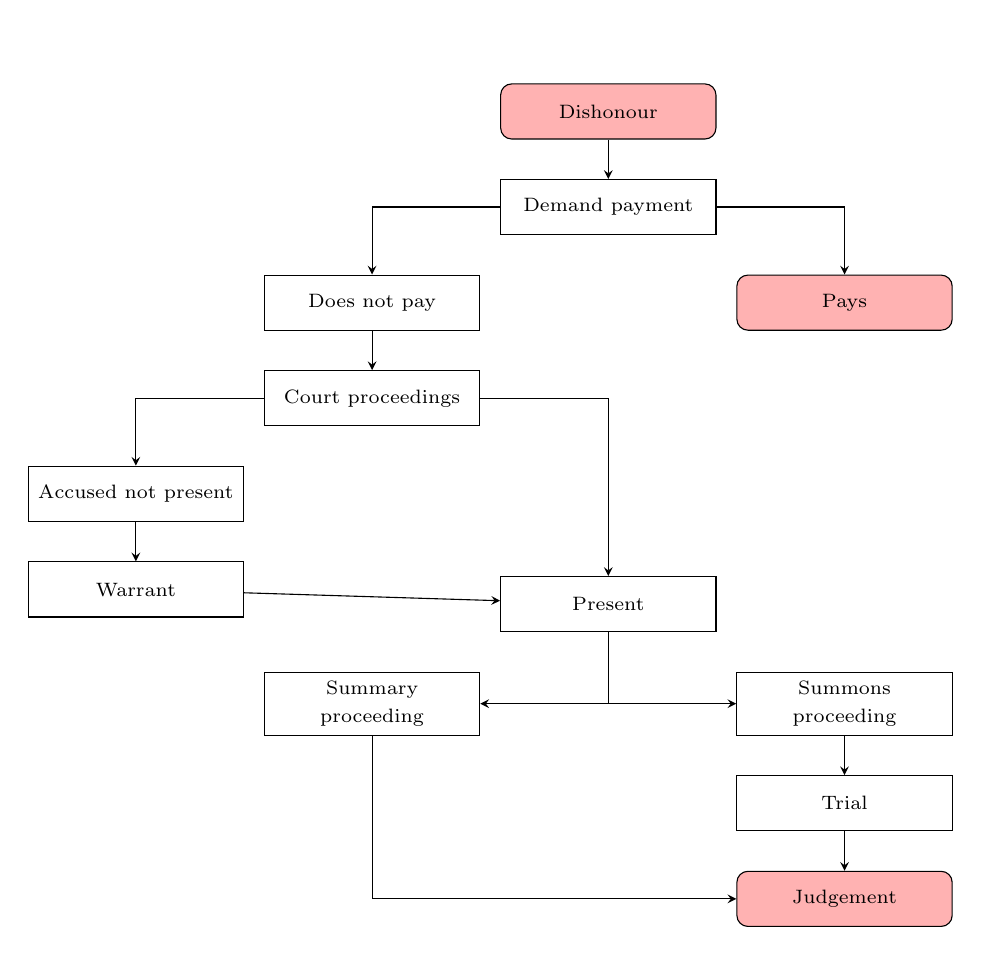
\begin{tikzpicture}[node distance= 1cm, text width=2.5cm]
\node (in0) [note] {};
\node (in1) [main, fill=red!30, below = 0.5cm of in0, yshift = 0.8cm] {Dishonour};
\node (in2) [process, below = 0.5cm of in1] {Demand payment};
\node (in3) [process, below = 0.5cm of in2, xshift = -3cm] {Does not pay};
\node (in4) [main, fill=red!30, below = 0.5cm of in2, xshift = 3cm] {Pays};
\node (in5) [process, below = 0.5cm of in3]{Court proceedings};
\node (in6) [process, below = 0.5cm of in5, xshift = -3cm] {Accused not present};
\node (in7) [process, below = 0.5cm of in6] {Warrant};
\node (in8) [process, below = 1.9cm of in5, xshift = 3cm] {Present};
\node (in9) [process, below = 0.5cm of in8, xshift = -3cm] {Summary proceeding};
\node (in10) [process, below = 0.5cm of in8, xshift = 3cm] {Summons proceeding};
\node (in11) [process, below = 0.5cm of in10] {Trial};
\node (in12) [main, fill=red!30, below = 0.5cm of in11] {Judgement};

\draw [arrow] (in1) -- (in2);
\draw [arrow] (in2) -| (in3);
\draw [arrow] (in2) -| (in4);
\draw [arrow] (in3) -- (in5);
\draw [arrow] (in5) -| (in6);
\draw [arrow] (in5) -| (in8);
\draw [arrow] (in6) -- (in7);
\draw [arrow] (in7) -- (in8);
\draw [arrow] (in8) |- (in9);
\draw [arrow] (in8) |- (in10);
\draw [arrow] (in10) -- (in11);
\draw [arrow] (in11) -- (in12);
\draw [arrow] (in9) |- (in12);

\end{tikzpicture}
\end{figure}

%%% Local Variables:
%%% mode: latex
%%% TeX-master: "paper_chequeDishonour"
%%% End:
\end{appendices}

\newpage
\printbibliography[heading=bibintoc]

\end{document}

%%% Local Variables:
%%% mode: latex
%%% TeX-master: t
%%% End: